%%%%%%%%%%%%%%%%%%%%%%%%%%%%%%%%%%%%%%%%%%%%%%%%%%%%%%%%%%%%%%%%%%%%%%%%%%%%%%%%
%2345678901234567890123456789012345678901234567890123456789012345678901234567890
%        1         2         3         4         5         6         7         8

% \documentclass[letterpaper, 10 pt, conference]{ieeeconf}  % Comment this line out if you need a4paper

\documentclass[a4paper, 10pt, conference]{ieeeconf}      % Use this line for a4 paper

\IEEEoverridecommandlockouts                              % This command is only needed if 
                                                          % you want to use the \thanks command

\overrideIEEEmargins                                      % Needed to meet printer requirements.

\usepackage[utf8]{inputenc}
\usepackage{graphicx}
\usepackage{listings}

\title{\LARGE \bf
Sistema Multi-Robôs para Cobertura Eficiente de Ambientes Domésticos
}


\author{Bernardo Borges e Daniele Diniz}


\begin{document}



\maketitle
\thispagestyle{empty}
\pagestyle{empty}


%%%%%%%%%%%%%%%%%%%%%%%%%%%%%%%%%%%%%%%%%%%%%%%%%%%%%%%%%%%%%%%%%%%%%%%%%%%%%%%%
\section{INTRODUÇÃO}

\subsection{Contextualização}

Uma aplicação relevante na área de robótica é a dos robôs aspiradores, que têm a
função de percorrer o ambiente doméstico de forma autônoma, recolhendo detritos
ao longo do caminho. Este projeto abordará o problema de cobertura no contexto de
sistemas multi-robôs, com o objetivo de dividir a tarefa entre dois robôs. Um dos
principais desafios nesta área é garantir que os robôs executem seu trajeto de forma
eficiente, evitando a movimentação aleatória pelo espaço, como observado em
robôs aspiradores convencionais, conforme demonstrado no vídeo da Neato
Robotics.

\begin{figure}[htb!]
    \centering
    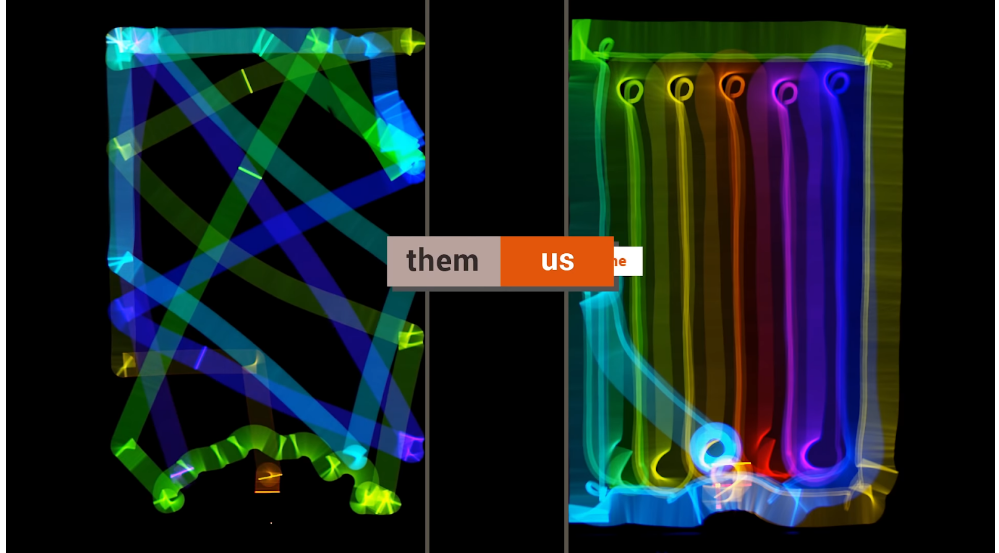
\includegraphics[scale=0.23]{./images/neato_compare.png}
    \caption{Comparativo de robôs apiradores sem e com planejamento de caminhos}
    \label{fig:fig9}
\end{figure}

Para superar esses desafios, utilizaremos nosso conhecimento em mapeamento,
controle e algoritmos para desenvolver um sistema de multi-robôs que abordará o
problema de cobertura do ambiente de forma eficaz, completa e, adicionalmente,
enfrentaremos o desafio de implementar a colaboração entre os robôs. A
implementação será realizada utilizando a linguagem Python e o simulador
CoppeliaSim.


\subsection{Motivação}

Abordar este problema é crucial para aumentar a eficiência energética e reduzir a
pegada de carbono dos robôs aspiradores domésticos. Um planejamento adequado
permite que esses robôs executem suas tarefas de maneira mais rápida e eficiente,
contribuindo significativamente para a sustentabilidade ambiental. As principais
aplicações incluem a limpeza autônoma em residências, escritórios e outros
espaços fechados onde a manutenção regular é necessária.

\subsection{Descrição do Problema}

O problema específico abordado é a ineficiência dos trajetos dos robôs aspiradores
domésticos devido à ausência de um planejamento deliberativo de cobertura. Os
desafios incluem a criação de um mapa da residência, a discretização do ambiente
em uma grade, e a implementação de algoritmos de cobertura que permitam a
coordenação eficiente de múltiplos robôs. O objetivo é desenvolver uma solução
que possibilite aos robôs realizar trajetos otimizados e colaborativos, minimizando o
tempo e a energia consumidos para limpar o ambiente completamente.
Em nossa implementação, consideraremos um ambiente com dois robôs que devem
colaborar na limpeza, de forma paralela. Além disso, vamos trabalhar partindo de
um mapa pré-existente do ambiente, que teria sido obtido em uma fase anterior, no
caso de uma implementação real.

\section{TRABALHOS RELACIONADOS}

Implementações similares ao nosso projeto incluem os robôs da Neato Robotics.
Esses robôs utilizam técnicas de mapeamento e navegação com base em visão computacional
(bitvision) e empregam modelos treinados com florestas aleatórias para melhorar a eficiência da navegação
e da cobertura do ambiente.

Diversos estudos abordam o problema de cobertura em sistemas multi-robôs.
Um exemplo relevante é o artigo "Exact and Heuristic Multi-Robot Dubins Coverage Path Planning for Known Environments"
publicado na revista Sensors.
Este estudo apresenta métodos exatos e heurísticos para o planejamento de trajetórias de cobertura
para múltiplos robôs em ambientes conhecidos.
A pesquisa destaca a importância de criar trajetórias eficientes que minimizem o tempo e os
recursos necessários para a cobertura completa do ambiente, focando em trajetórias do tipo
Dubins, que são especialmente úteis para robôs com restrições de movimentação como os robôs aspiradores.

\begin{figure}[htb!]
    \centering
    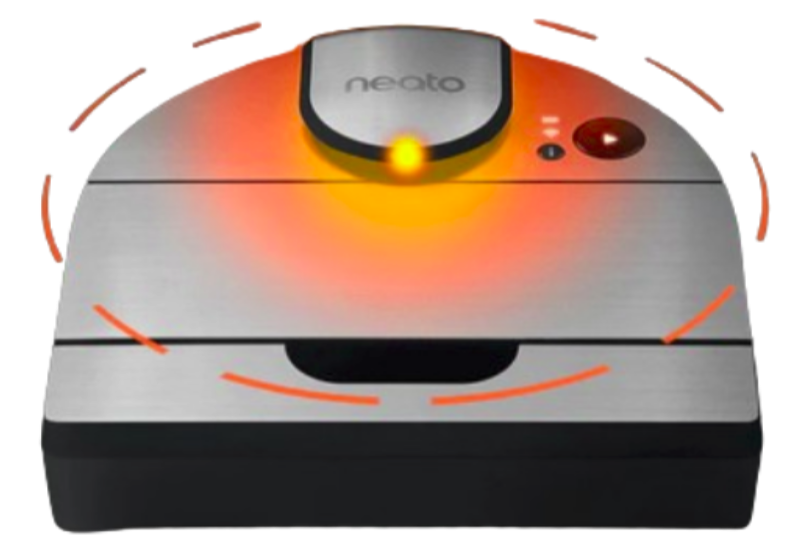
\includegraphics[scale=0.2]{./images/neato_bot.png}
    \caption{Robô aspirador da empresa Neato Robotics}
\end{figure}


\newpage

\section{METODOLOGIA}
% descrição detalhada sobre a implementação. Deve ser discutido as estruturas de
% dados e algoritmos utilizados, bem como decisões tomadas relativas aos casos e detalhes que
% porventura estejam omissos no enunciado.

Pensando em todos os problemas apresentados, trazemos uma solução que realizará um
\textbf{mapeamento assertivo} para obter uma cobertura eficiente, realizando a delimitação
de áreas de atuação dos robôs, o que evitará problemas de colisão entre eles.

\subsection{Premissas}
Para nosso projeto realizamos algumas suposições:
\begin{itemize}
    \item O mapa do ambiente é conhecido;
    \item Os robôs conseguem se comunicar;
    \item O ambiente será \textbf{discretizado}, em células ocupadas($1$) e desocupadas ($0$);
\end{itemize}

\subsection{Separação de Tarefas}
Considerando os múltiplos robôs, iremos atribuir regiões disjuntas para atuação.
Para isso utilizaremos o algoritmo \textbf{Flood Fill}, que partirá de dois extremos
do mapa e irá pintá-lo de \textit{vermelho} e \textit{azul} para as duas regiões.

\lstset{language=Python}
\begin{lstlisting}
def create_job_division():
    s0 = find_first_free_cell()
    sf = find_last_free_cell()
    queue = [s0,sf]
    while not queue.empty:
        (i,j,c) = queue.pop()
        if ColorGraph[i][j] != UNSET:
            continue
        ColorGraph[i][j] = c
        for (di,dj) in connect4Moves:
            if not valid cell (di,dj):
                continue
            q.append((di,dj,c))
        
\end{lstlisting}

Após esse algortimo, conseguimos as regiões para cada robô:

\begin{figure}[htb!]
    \centering
    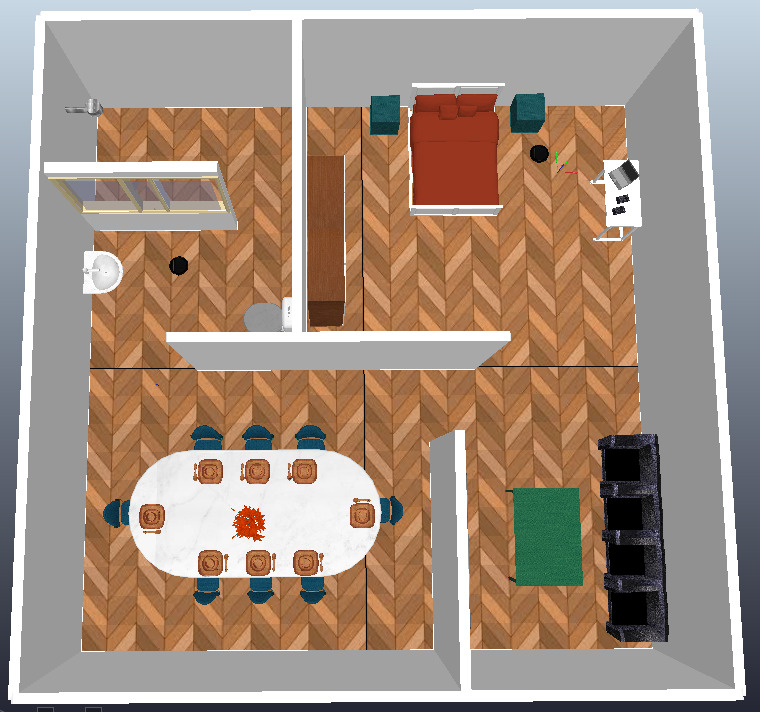
\includegraphics[scale=0.2]{../home_pic.png}
    \caption{Imagem aérea da cena "home"}
\end{figure}


\begin{figure}[htb!]
    \centering
    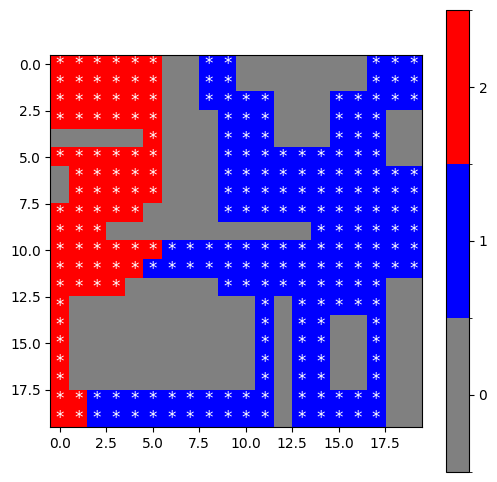
\includegraphics[scale=0.4]{../home_dirty.png}
    \caption{Divisão das regiões em vermelho e azul}
\end{figure}

\subsection{Robôs e Controle}
Para esse projeto usamos o robo "kobuki", que é direcional. 
O controle utilizado é "de Luca Oriolo" e utilizamos a locomoção 
inspirada em campos potênciais para criar uma força de atração do robô
em relação aos objetivos que vamos atualizando iterativamente.


\subsection{Navegação}

Para a navegação em alto nível implementamos uma lógica que visita células mais próxima primeiro,
ainda na lógica BFS:

\lstset{language=Python}
\begin{lstlisting}
for robot in robots:
    if robot.cells_left == 0: continue
    if robot.has_goal:
        robot.move_to_goal()
        continue
    [ri, rj] = robot.current_location
    for (dj, di) in moves:
        if robot.is_task_cell(ni, nj):
            robot.add_new_goal([ni,nj])
            break
    if robot.has_goal():
        robot.move_to_goal()
        continue
    # BFS to find nearest cell to clean
    path = robot.find_nearest_task_cell()
    if path == None: continue
    robot.add_new_goals(path)
    robot.move_to_goal()

\end{lstlisting}

Como podemos ver, primeiro tentamos limpar células na cruz de 4-conexão. Caso não haja
uma célula próxima realizamos uma BFS no grid, que passa por células pela cor atribuída
e seguimos esse caminho até o objetivo.


\section{RESULTADOS}

Conseguimos realizar nossos testes com sucesso em duas cenas distintas, a primeira se chama
"diningRoom" e possui uma grande mesa ao centro e bastantes células a serem cobertas. A segunda
cena é "home", um apartamento com quartos, sala e banheiro, que exige organização e precisão para limpeza

\begin{figure}[htb!]
    \centering
    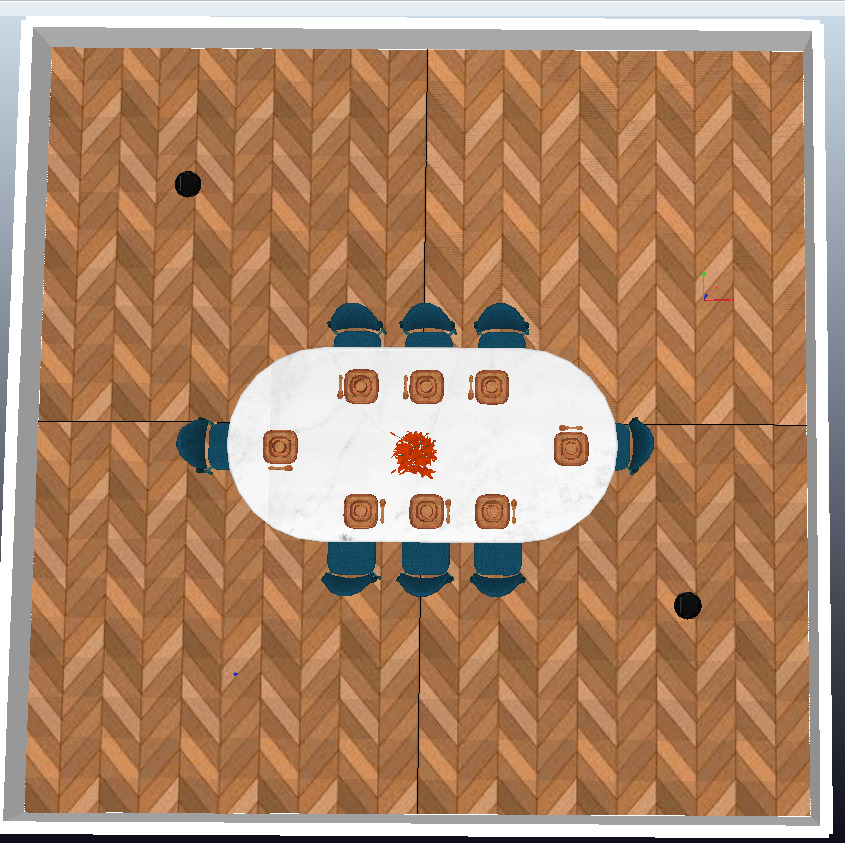
\includegraphics[scale=0.15]{../diner_pic.jpeg}
    \caption{Imagem aérea da cena "diningRoom"}
\end{figure}


\begin{itemize}
    \item Em \textit{DiningRoom} conseguimos coordenar os robôs para limpeza completa em 8 minutos e
          21 segundos.
          \begin{figure}[htb!]
              \centering
              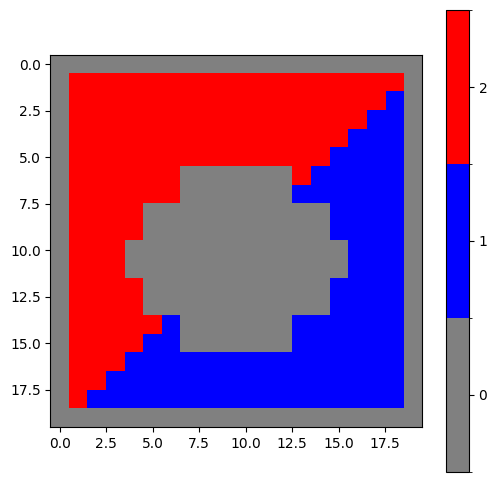
\includegraphics[scale=0.4]{../clean.png}
              \caption{Células limpas em \textit{DiningRoom}}
          \end{figure}
    \item Em \textit{Home} os robôs terminaram a limpeza em 7:38.
\end{itemize}


\newpage

\section{CONCLUSÃO}

Com esse trabalho conseguimos entender os problemas e soluções aplicadas na coordenação
de robôs, ainda que com apenas 2 elementos. Os desafios no ambiente de simulação foram de
localiazação, atribuição de tarefas, controle e organização de código, já que há mais peças
em movimento simultâneamente que deve ser pensadas.

Próximos passos possíveis para extender esse projeto serão:
\begin{itemize}
    \item Tranferência de tarefas, em um momento em que um robô terminou de limpar sua área, podera redividir a tarefa para não permanecer ocioso;
    \item Atualização Automática do Mapa, para cenários mais dinâmicos, como a mudança de móveis;
    \item Suporte para Diversos Robôs, aumentando a frota dinâmicamente dividindo a tarefa para mais robôs
\end{itemize}

\begin{thebibliography}{99}
    
    \bibitem{Li2023} H. Liu, ``Exact and Heuristic Multi-Robot Dubins Coverage Path Planning for Known Environments,'' \textit{Sensors}, vol. 23, no. 5, p. 2560, Feb. 2023. [Online]. Available: https://doi.org/10.3390/s23052560.
    
    
\end{thebibliography}




\end{document}
